\documentclass[dvipdfmx, border=10pt]{standalone}
\usepackage{amsmath}
\usepackage{amssymb}
\usepackage{tikz-cd}

\begin{document}
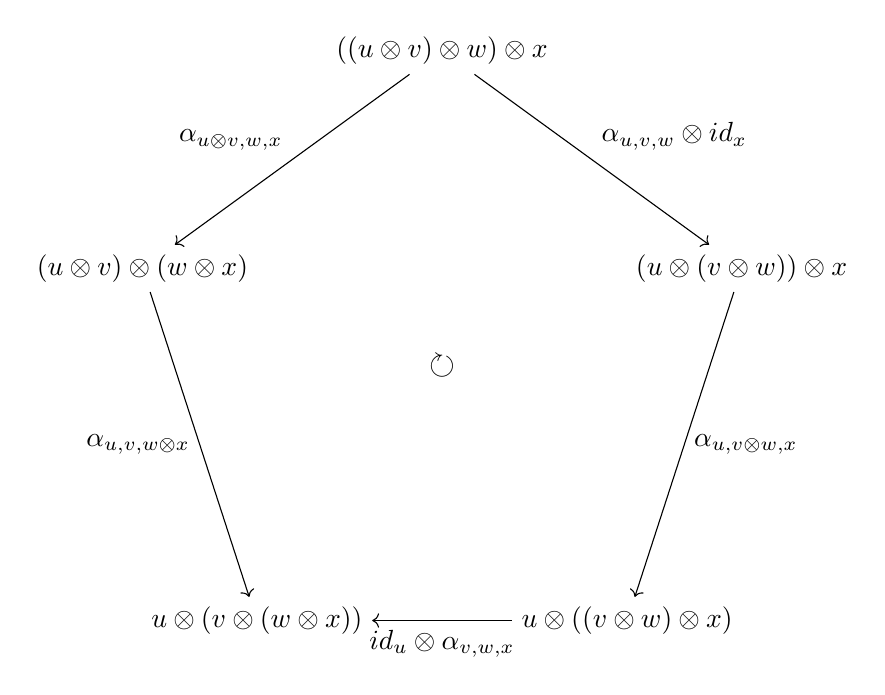
\begin{tikzpicture}[commutative diagrams/every diagram]
  \node (N1) at (90:4cm)  {$((u \otimes v) \otimes w) \otimes x$};
  \node (N2) at (162:4cm) {$(u \otimes v) \otimes (w \otimes x)$};
  \node (N3) at (234:4cm) {$u \otimes (v \otimes (w \otimes x))$};
  \node (N4) at (306:4cm) {$u \otimes ((v \otimes w) \otimes x)$};
  \node (N5) at (18:4cm)  {$(u \otimes (v \otimes w)) \otimes x$};
  \path[->] (N1) edge node[above left] {$\alpha_{u\otimes v, w, x}$} (N2);
  \path[->] (N2) edge node[left]       {$\alpha_{u, v, w\otimes x}$} (N3);
  \path[->] (N1) edge node[above right] {$\alpha_{u,v,w} \otimes id_x$} (N5);
  \path[->] (N5) edge node[right]       {$\alpha_{u, v\otimes w, x}$} (N4);
  \path[->] (N4) edge node[below] {$id_u \otimes \alpha_{v,w,x}$} (N3);
  \node at (0,0) {\large $\circlearrowright$};
\end{tikzpicture}
\end{document}